%-----------------------------------------------------------------------
% Functional Programming 4
% John O'Donnell, Wim Vanderbauwhede
% University of Glasgow
%-----------------------------------------------------------------------

\documentclass{beamer}
\usepackage{jtodlecseriesFP4}
%include polycode.fmt
%format alpha = "\alpha"
%format ~> = "\leadsto "

% Identify this presentation
\SetPresentationTitle
  {Returning Functions as Values -- Parsing}
  {Returning Functions as Values -- Parsing}
\SetPresentationNumber
  {7}
\SetPresentationDate
  {Week 4-1}
  {Week 4-1}

%-----------------------------------------------------------------------

% Beginning

\begin{document}

\begin{frame}[fragile]
  \PresentationTitleSlide
\end{frame}


%-----------------------------------------------------------------------

\begin{frame}[fragile]
  \frametitle{Topics}
  \tableofcontents
\end{frame}
%-----------------------------------------------------------------------
\section{The Parsing Problem}
\begin{frame}[fragile]
\begin{center}
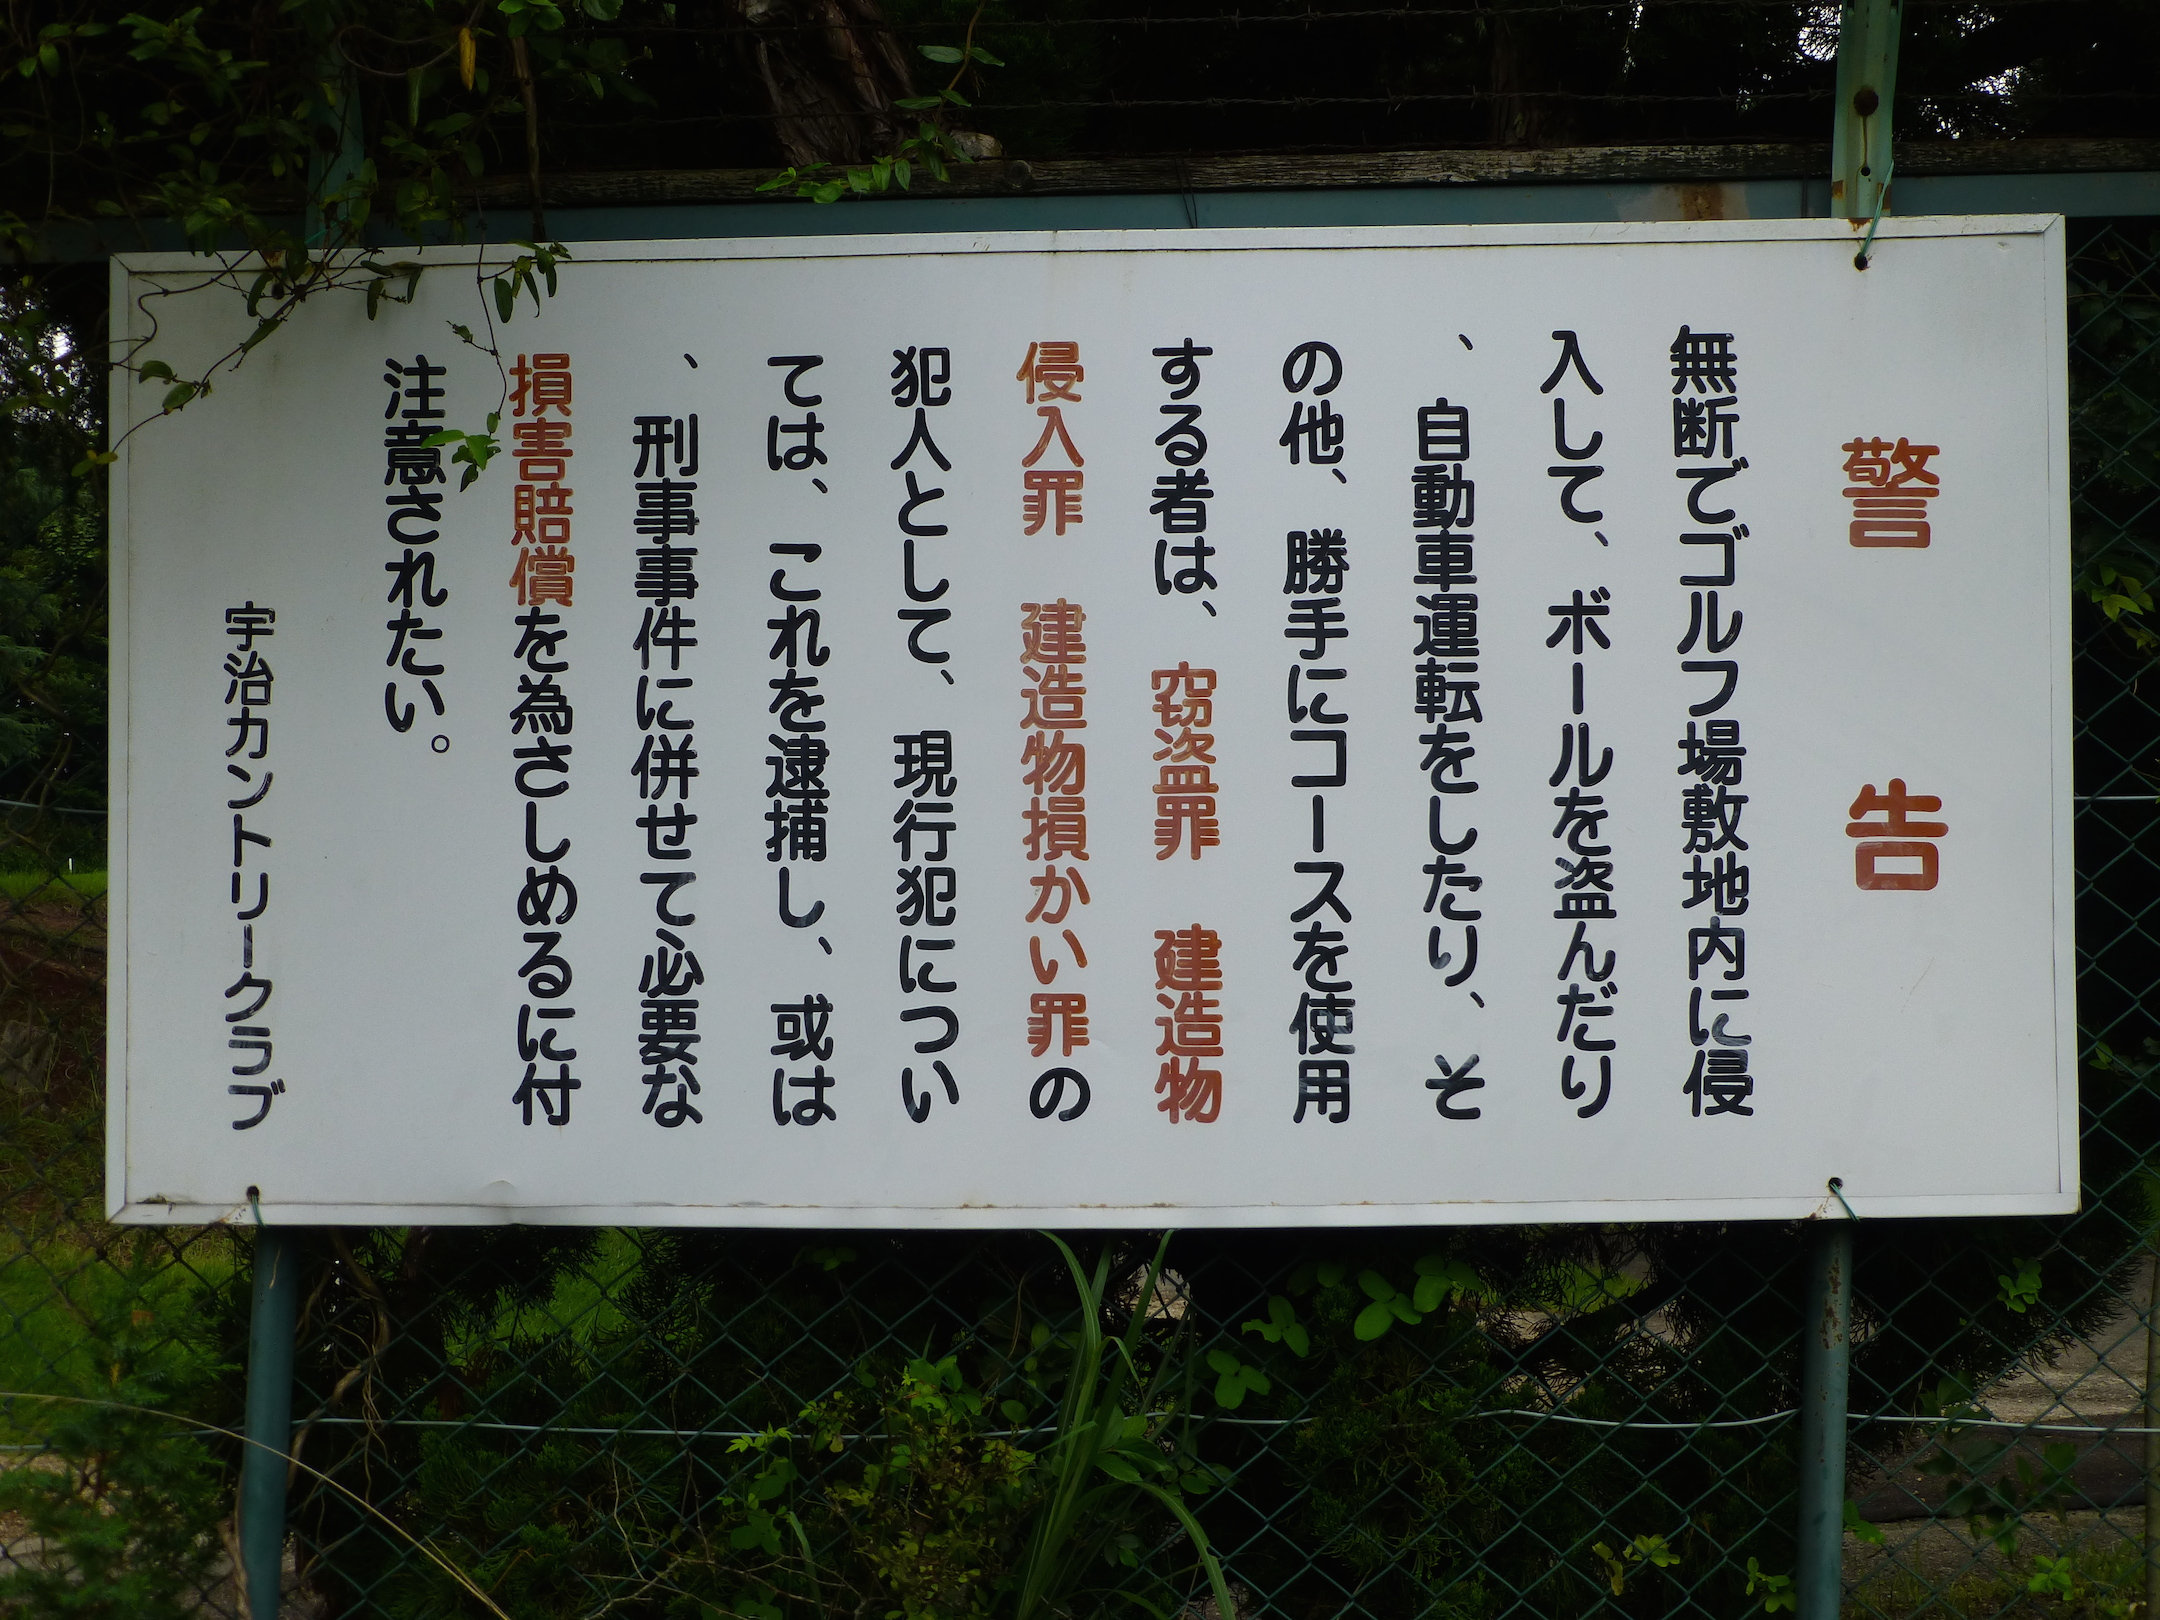
\includegraphics[scale=0.35]
    {figures/jpg/pic05.jpg}
\end{center}
\end{frame}

%-----------------------------------------------------------------------

\section{Returning functions as values}

\begin{frame}[fragile]
\frametitle{Returning functions as values}

\begin{itemize}
\item So far, we have seen functions that take functions as arguments
\item Functions can also return  functions as values
\item For example, partial application of a function:

\begin{verbatim}
sum = foldl (+) 0
\end{verbatim}

Here $sum$ is the result returned by  partial application of $foldl$.

\item More explicitly, we can write this as:

\begin{verbatim}
sum = \xs -> foldl (+) 0 xs
\end{verbatim}

Here $sum$ is a function resulting from partial application of $foldl$.

\item Both are of course the same thing, just different interpretations.
\end{itemize}
\end{frame}

%-----------------------------------------------------------------------

\section{Function generators}

\begin{frame}[fragile]
\frametitle{Function generators}

\begin{itemize}
\item We can use this to generate parametrised functions

\begin{verbatim}
gen_add_n = \n ->
    \x -> x+n
	
add_3 = gen_add_n 3	
add_7 = gen_add_n 7

add_3 5 --> 8
add_7 4 --> 11
\end{verbatim}

\item This is of course not limited to numeric constants:

\begin{verbatim}
gen_op_n = \op n ->
    \x -> x `op` n
	
add_3 = gen_op_n (+) 3	
mult_7 = gen_op_n (*) 7

add_3 5 --> 8
mult_7 4 --> 28
\end{verbatim}

\end{itemize}
\end{frame}


%-----------------------------------------------------------------------
\section{Structuring a program}
\begin{frame}
\frametitle{Structuring a program} 

\begin{enumerate}
\item Design an algebraic data type as your main data
  representation.
\item Define some test cases, just using the constructors of the
  type.
\item Develop the core functionality of your program: this may take
  the form of tree traversals, or tree transformations.
\item Develop a prototype implementation, using $read$ and $show$
  to convert between strings and your algebraic data type.
\item Later, add a parser for reading input just the way you want
  it, and write your own $show$ functions to format the output.
\end{enumerate}

\end{frame}
%-----------------------------------------------------------------------
\begin{frame}[fragile]
\frametitle{Cooking soba noodles}
\begin{quote}

Bring a large pot of water up to a boil. Unlike Italian pasta, you do not need to salt the water. Once it's boiling, hold the noodles over the water and sprinkle them in strand by strand.
Once all the noodles are in, stir gently so that they are all immersed in the water.
Bring the water back up to a gentle boil, then lower the heat so that the water is just simmering. (This differs from the 'rolling boil' that's recommended for pasta.) If the water threatens to boil over, add about 1/2 cup of cold water (but if you lower the heat to the gentle simmer, and have a big enough pot, this shouldn't be necessary). Cook for about 7 to 8 minutes, or following the package directions (for thinner noodles 5 to 6 minutes may be enough. Test by eating a strand - it should be cooked through, not al dente, but not mushy either).

\end{quote}

\end{frame}



%-----------------------------------------------------------------------
\section{Parsing text}
\begin{frame}[fragile]
\frametitle{Parsing text}

\begin{enumerate}
\item Typically, a functional program is organised around a tree-like data structure with an algebraic data type that represents the core data
\item A parser reads text input and generates the tree
\item Functions perform transformations or traversals on the tree
\item Pretty-printer functions output the tree (original or transformed)
\end{enumerate}
\end{frame}

%-----------------------------------------------------------------------

\begin{frame}[fragile]
\frametitle{Alternative approaches to parsing}

\begin{itemize}
\item Don't bother with parsing, just make the user provide in put
  in an awkward form.  \emph{A common approach, but please don't do
    this!}
\item Write the parser by hand, with just ordinary list processing
  functions. Possible, but hard and not reusable. Don't do it.
\item Write the parser using \emph{regular expressions}. Tempting but limiting and not reusable. Don't do it, unless your input text format is very simple.  
\item Use \emph{parser combinators}.  For most
  purposes, this is the recommended approach, for everything from
  basic input formats to medium size programming languages   (e.g. Pascal) or subsets of languages like C and Fortran.
\item Use a parser generator, e.g. \emph{bison, antlr, happy}.  The best approach
  for heavy-weight parsers, for very large programming languages.
\end{itemize}
\end{frame}

%-----------------------------------------------------------------------
\begin{frame}[fragile]
\frametitle{Parser combinators}

\begin{itemize}
\item Parser combinators are functions that allow you to combine smaller parsers into bigger ones.
\item They are higher-order functions that take functions as arguments and return functions
\item A parser combinator library provides both basic parsers (for words, numbers etc.) and combinators.
\end{itemize}

\end{frame}
%-----------------------------------------------------------------------
\begin{frame}[fragile]
\frametitle{Parsec: monadic parsing combinators}

\begin{itemize}
\item There are many parsing libraries for Haskell.
\item One of the most widely used is Parsec, which is robust,
  flexible, expressive, and efficient.
\item Parsec operates in a monad.
\end{itemize}

\end{frame}

%-----------------------------------------------------------------------
\begin{frame}[fragile]
\frametitle{Form of a parser}

\begin{itemize}
\item For example, suppose we want to  parse a string of the form $<tag>$, where
  $tag$ must be a word, and return the tag as a type $Tag$.


\begin{verbatim}
data Tag = MkTag String

parseTag :: Parser Tag
parseTag =
  do  char '<'
      x <- identifier
      char '>'
      return (MkTag x)
\end{verbatim}

\end{itemize}

\end{frame}

%-----------------------------------------------------------------------
\begin{frame}[fragile]
\frametitle{Testing a parser}

{\footnotesize
\begin{verbatim}
[wim@fp4 ~]$ ghci
GHCi, version 7.4.1: http://www.haskell.org/ghc/  :? for help
Loading package ghc-prim ... linking ... done.
Loading package integer-gmp ... linking ... done.
Loading package base ... linking ... done.
Prelude> import Text.ParserCombinators.Parsec
Prelude Text.ParserCombinators.Parsec> parseTest (char 'b') "cons"
Loading package bytestring-0.9.2.1 ... linking ... done.
Loading package transformers-0.2.2.0 ... linking ... done.
Loading package mtl-2.0.1.0 ... linking ... done.
Loading package array-0.4.0.0 ... linking ... done.
Loading package deepseq-1.3.0.0 ... linking ... done.
Loading package text-0.11.2.0 ... linking ... done.
Loading package parsec-3.1.2 ... linking ... done.
parse error at (line 1, column 1):
unexpected "c"
expecting "b"
Prelude Text.ParserCombinators.Parsec> parseTest (char 'c') "cons"
'c'
Prelude Text.ParserCombinators.Parsec> 

\end{verbatim}
}

\end{frame}
%-----------------------------------------------------------------------
\begin{frame}[fragile]
\frametitle{Running the parser}

{\footnotesize
\begin{verbatim}
*Main> run parseTag "<div>"
Loading package parsec-2.1.0.1 ... linking ... done.
MkTag "div"
\end{verbatim}
}

{\footnotesize
\begin{verbatim}
*Main> run parseTag "div"
parse error at (line 1, column 1):
unexpected "d"
expecting "<"
*Main> 

\end{verbatim}
}

\end{frame}
%-----------------------------------------------------------------------
\begin{frame}[fragile]
\frametitle{Anatomy of a basic parser}

\begin{itemize}
\item All parser combinators are functions that return functions.
\item It is the returned function that operates on the string, not the parser combinator function.
\item The basic parsers ($identifier$,$natural$,$char$) take either no arguments (e.g. $identifier$) or one or more strings for parametrisation (e.g. $char$). 

\begin{verbatim}
char = \ch -> \str ->
      -- try to match the character ch
      -- return the result
\end{verbatim}
If the match succeeds, the matching string is removed from the input string; otherwise, the original string is returned, e.g.
\begin{verbatim}
char 'c' "cons" -->
'c'
char 'b' "cons" --> 
parse error at (line 1, column 1):
unexpected "c"
expecting "b"
\end{verbatim}
\end{itemize}   
\end{frame}

%-----------------------------------------------------------------------
\begin{frame}[fragile]
\frametitle{Anatomy of a parser combinator}

\begin{itemize}
\item Parser combinators such as $<|>$ and $parens$ take other parsers as arguments. 

\begin{verbatim}
parens = \p ->
    \str ->
        -- first match '('
        -- perform the parse of p if '(' was found
        -- then match ')'
        -- return the result
\end{verbatim}

\end{itemize}   
\end{frame}


%-----------------------------------------------------------------------
\begin{frame}[fragile]
\frametitle{Parsing alternatives}

\begin{itemize}
\item Often we want to try one parser; if that fails, then try
  another one instead. The choice combinator \texttt{<|>} provides this functionality. 
\item Example: $letter\_digit$ will match either a letter or a
  digit.

\end{itemize}


\begin{verbatim}
letter_digit :: Parser Char
letter_digit =
  do  x <- letter <|> digit
      return x
\end{verbatim}

\end{frame}



%-----------------------------------------------------------------------

%-----------------------------------------------------------------------
\begin{frame}[fragile]
\frametitle{Running alternative parsers}

{\footnotesize
\begin{verbatim}
*Main> run letter_digit "b2"
'b'
\end{verbatim}
}

{\footnotesize
\begin{verbatim}
*Main> run letter_digit "2b"
'2'
\end{verbatim}
}

{\footnotesize
\begin{verbatim}
*Main> run letter_digit "*2"
parse error at (line 1, column 1):
unexpected "*"
expecting letter or digit
\end{verbatim}
}

\end{frame}

%-----------------------------------------------------------------------
\begin{frame}[fragile]
\frametitle{Parsing alternative strings}

Suppose we want to match either \emph{bag} or \emph{bog}, but nothing else.

\begin{verbatim}
bag_bog :: Parser String
bag_bog =
  do  xs <- string "bag" <|> string "bog"
      return xs
   \end{verbatim}

\end{frame}

%-----------------------------------------------------------------------
\begin{frame}[fragile]
\frametitle{Failed alternative consumes input}

So far so good:

{\footnotesize
\begin{verbatim}
*Main> run bag_bog "bag"
"bag"
\end{verbatim}
}

And a non-matching string fails, as expected.

{\footnotesize
\begin{verbatim}
*Main> run bag_bog "bug"
parse error at (line 1, column 1):
unexpected "u"
expecting "bag"
\end{verbatim}
}

But there's a problem!

{\footnotesize
\begin{verbatim}
*Main> run bag_bog "bog"
parse error at (line 1, column 1):
unexpected "o"
expecting "bag"
\end{verbatim}
}

The first parser \emph{string "bag"} matched the \texttt{b} but then failed on
the \texttt{a}.  \emph{It has now consumed the \texttt{b}.}  The second parser
\emph{string "bog"} now tries to match \texttt{b}against\texttt{o}, which of course
fails.

\end{frame}

%-----------------------------------------------------------------------
\begin{frame}[fragile]
\frametitle{try --- don't consume input on failed parse}

\begin{verbatim}
bag_bog_try :: Parser String
bag_bog_try =
  do  xs <- try (string "bag") <|> string "bog"
      return xs
\end{verbatim}

\end{frame}

%-----------------------------------------------------------------------
\begin{frame}[fragile]
\frametitle{Trying a parse without consuming input}

{\footnotesize
\begin{verbatim}
*Main> run bag_bog_try "bag"
"bag"
\end{verbatim}
}

{\footnotesize
\begin{verbatim}
*Main> run bag_bog_try "bug"
parse error at (line 1, column 1):
unexpected "u"
expecting "bog"
\end{verbatim}
}

{\footnotesize
\begin{verbatim}
*Main> run bag_bog_try "bog"
"bog"
\end{verbatim}
}

\end{frame}

%-----------------------------------------------------------------------

%-----------------------------------------------------------------------
\begin{frame}[fragile]
\frametitle{Some parsers from the library}

The Parsec library provides some  small parsers that are useful for
defining bigger ones:

\begin{itemize}
\item $char\; '?'$ --- $char$ is applied to a character, and it gives a
  parser that matches that character  
\item $letter$ --- matches any letter
\item $digit$ --- matches any digit
\item $string$ --- matches a string of characters
\item $stringLiteral\; "xyz*"$ --- matches the string argument
\item $many\; p$ --- matches 0 or more occurrences of parser $p$
\item $many1\; p$ --- matches 1 or more occurrences of parser $p$
\end{itemize}

\end{frame}

% -----------------------------------------------------------------------
\begin{frame}[fragile]
\frametitle{Variable names}

\begin{verbatim}
varname :: Parser String
varname =
  do  x <- letter
      xs <- many (letter <|> digit)
      return (x:xs)
\end{verbatim}

{\footnotesize
\begin{verbatim}
*Main> run varname "a4cc7*5"
"a4cc7"
*Main> run varname "34a"
parse error at (line 1, column 1):
unexpected "3"
expecting letter
\end{verbatim}
}

\end{frame}
% -----------------------------------------------------------------------
\begin{frame}[fragile]
\frametitle{Expression parsers}
\begin{itemize}
\item Arithmetic expressions are complex to parse because of the rules of precedence and the arity of the operators.
\item Parsec provides support for expression parsing, so you don't have to write your own expression parser.
\end{itemize}

{\footnotesize
\begin{verbatim}
expr_parser :: Parser Expr
expr_parser = buildExpressionParser optable term <?> "expression"

optable =
  let
    op name assoc   = 
      Infix ( do {  reservedOp name; 
          return (\x y ->(Op (MkOpExpr name x y))) } ) assoc
    prefix name = 
      Prefix  ( 
        reservedOp name >> 
            return (\x->(Pref (MkPrefixOpExpr name x))) ) 
  in
    [ [ op "*"  AssocLeft, op "/"  AssocLeft, op "%" AssocLeft ]
    , [ op "+"  AssocLeft, op "-"  AssocLeft ], [ prefix "-" ] ]

\end{verbatim}
}

\end{frame}

\begin{frame}[fragile]
\frametitle{Expression parsers}
\begin{itemize}
\item Parsec also has support for programming languages with a mechanism to define the syntax and keywords through \emph{makeTokenParser}. 
\item For simple cases, you can use \emph{emptyDef}.
\end{itemize}

{\footnotesize
\begin{verbatim}
import Text.ParserCombinators.Parsec.Expr
import qualified Text.ParserCombinators.Parsec.Token as P
lexer       = P.makeTokenParser emptyDef    

parens          = P.parens lexer    
commaSep        = P.commaSep lexer
-- and many more 
\end{verbatim}
}

\end{frame}


\end{document}
